\documentclass{classrep}
\usepackage[utf8]{inputenc}
\usepackage{color}
\usepackage{graphicx}

\DeclareUnicodeCharacter{00A0}{~}

\studycycle{Informatyka, studia dzienne, inż I st.}
\coursesemester{VI}

\coursename{Sztuczna inteligencja i systemy ekspertowe}
\courseyear{2019/2020}

\courseteacher{Krzysztof Lichy}
\coursegroup{poniedziałek, 10:15}

\author{
  \studentinfo{Paweł Białek}{216723} \and
  \studentinfo{Łukasz Kostrzewa}{216804}
}

\title{Zadanie 1: Piętnastka}

\begin{document}
\maketitle


\section{Cel}
{\color{black}
Celem zadania było napisanie programu rozwiązującego układankę zwaną "Piętnastką" za pomocą różnych metod przeszukiwania. Następnie należało dokonać porównania
skuteczności wszystkich analizowanych metod.}

\section{Wprowadzenie}
{\color{black}
Piętnastka jest to układanka zbudowana z ramki 4x4  i znajdujących się w niej 15 elementów oznacza to, że możliwe jest przesuwanie niektórych elementów ponieważ w ramce pozostaje puste miejsce.
\begin{figure}
\centering
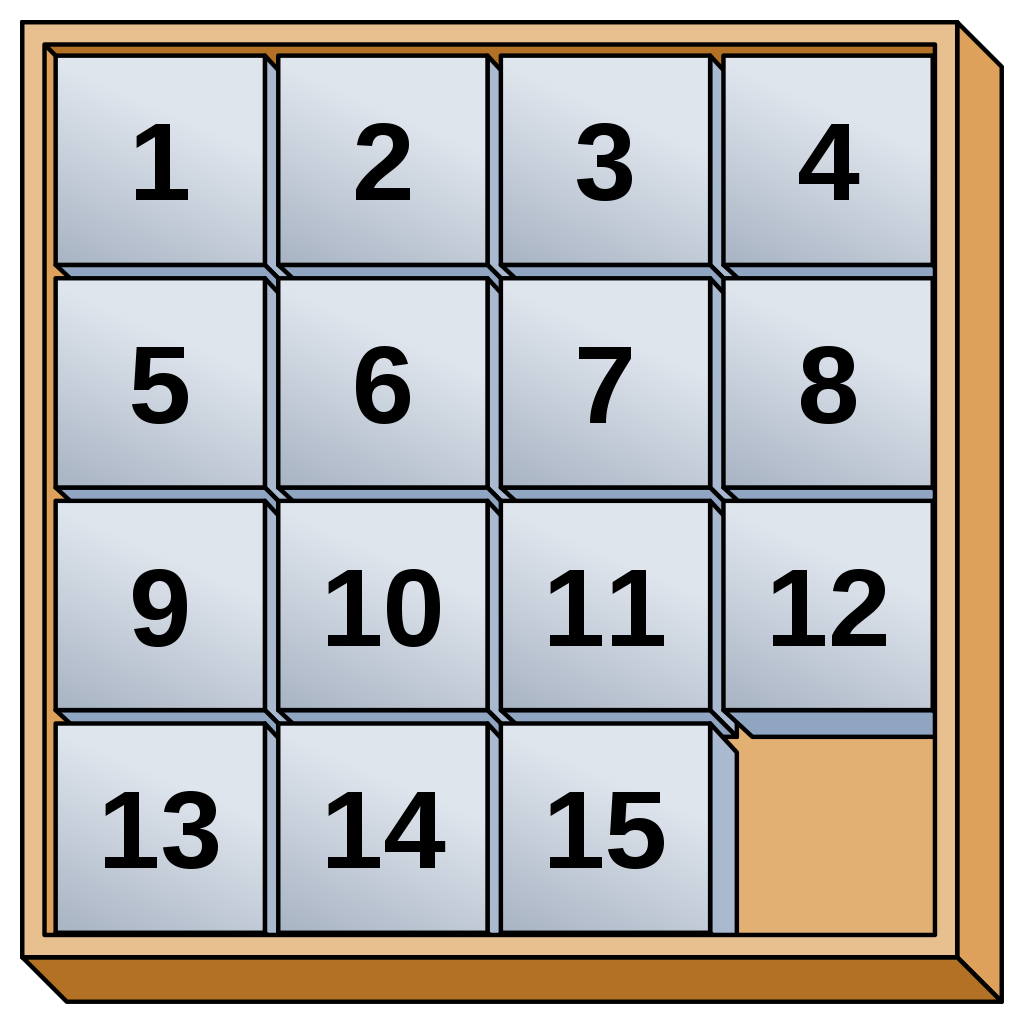
\includegraphics [scale=0.15]{1024px-15-puzzle.svg}
\caption{Rozwiązana układanka.}
\end{figure}
\newpage
W celu rozwiązania układanki użyto trzech metod przeszukiwania stanów:
\begin{enumerate}
\item Strategii przeszukiwania "wszerz" (BFS) - polega ona na przeszukiwaniu wszystkich wierzchołków na danym poziomie począwszy od stanu początkowego, po odwiedzeniu wszystkich wierzchołków przechodzi do następnego poziomu, aż do odnalezienia rozwiązania.
\item Strategii przeszukiwania "w głąb" (DFS) - polega ona na przeszukiwaniu wszystkich wierzchołków w danym korzeniu począwszy od stanu początkowego, po odwiedzeniu wszystkich wierzchołków przechodzi do następnego korzenia, aż do odnalezienia rozwiązania. 
\item Strategii "najpierw najlepszy": A*, z następującymi heurystykami: 
\begin{itemize}
\item metryką Hamminga - definicja
\item metryką Manhattan - definicja 
\end{itemize}
\end{enumerate}}

\section{Opis implementacji}
Program jest aplikacją konsolową napisaną w języku Java. Aby go uruchomić należy mieć zainstalowaną maszynę wirtualną javy oraz podać 5 parametrów podczas uruchamiania:
\begin{enumerate}
\item akronim określający wybraną strategię (bfs, dfs, astr)
\item dodatkowy parametr wybranej strategii:
\begin{itemize}
\item DFS I BFS - akronim liter R,L,U,D określający kolejność przeszukiwania (Right, Left, Up, Down)
\item A* - hamm dla heurystyki Hamminga, manh dla heurystyki Manhattan
\end{itemize}
\item nazwa pliku tekstowego z zadanym układem początkowym układanki
\item nazwa pliku tekstowego, w którym ma zostać zapisane rozwiązanie
\item nazwa pliku tekstowego, w którym mają zostać zapisane dodatkowe informacje dotyczące przeprowadzonego procesu obliczeniowego
\end{enumerate}
Na poniższym diagramie zaprezentowano strukturę aplikacji. Klasa Puzzle odpowiada za przechowywanie informacji o układzie planszy, a także pozwala na wyliczenie i wykonanie możliwych ruchów oraz porównanie przechowywanego układu do oczekiwanego układu. Klasy SolverBFS, SolverDFS i SolverAStar implementują algorytmy wykorzystywane do rozwiązywania puzzli zgodne z nazwą klasy. Klasy PuzzleLoader i PuzzleSaver odpowiadają odpowiednio za wczytanie planszy z odpowiednio skonstruowanego pliku oraz zapis do pliku wynikowego oraz pliku ze szczegółowymi informacjami o wykonaniu programu.
\newpage
\begin{figure}
\centering
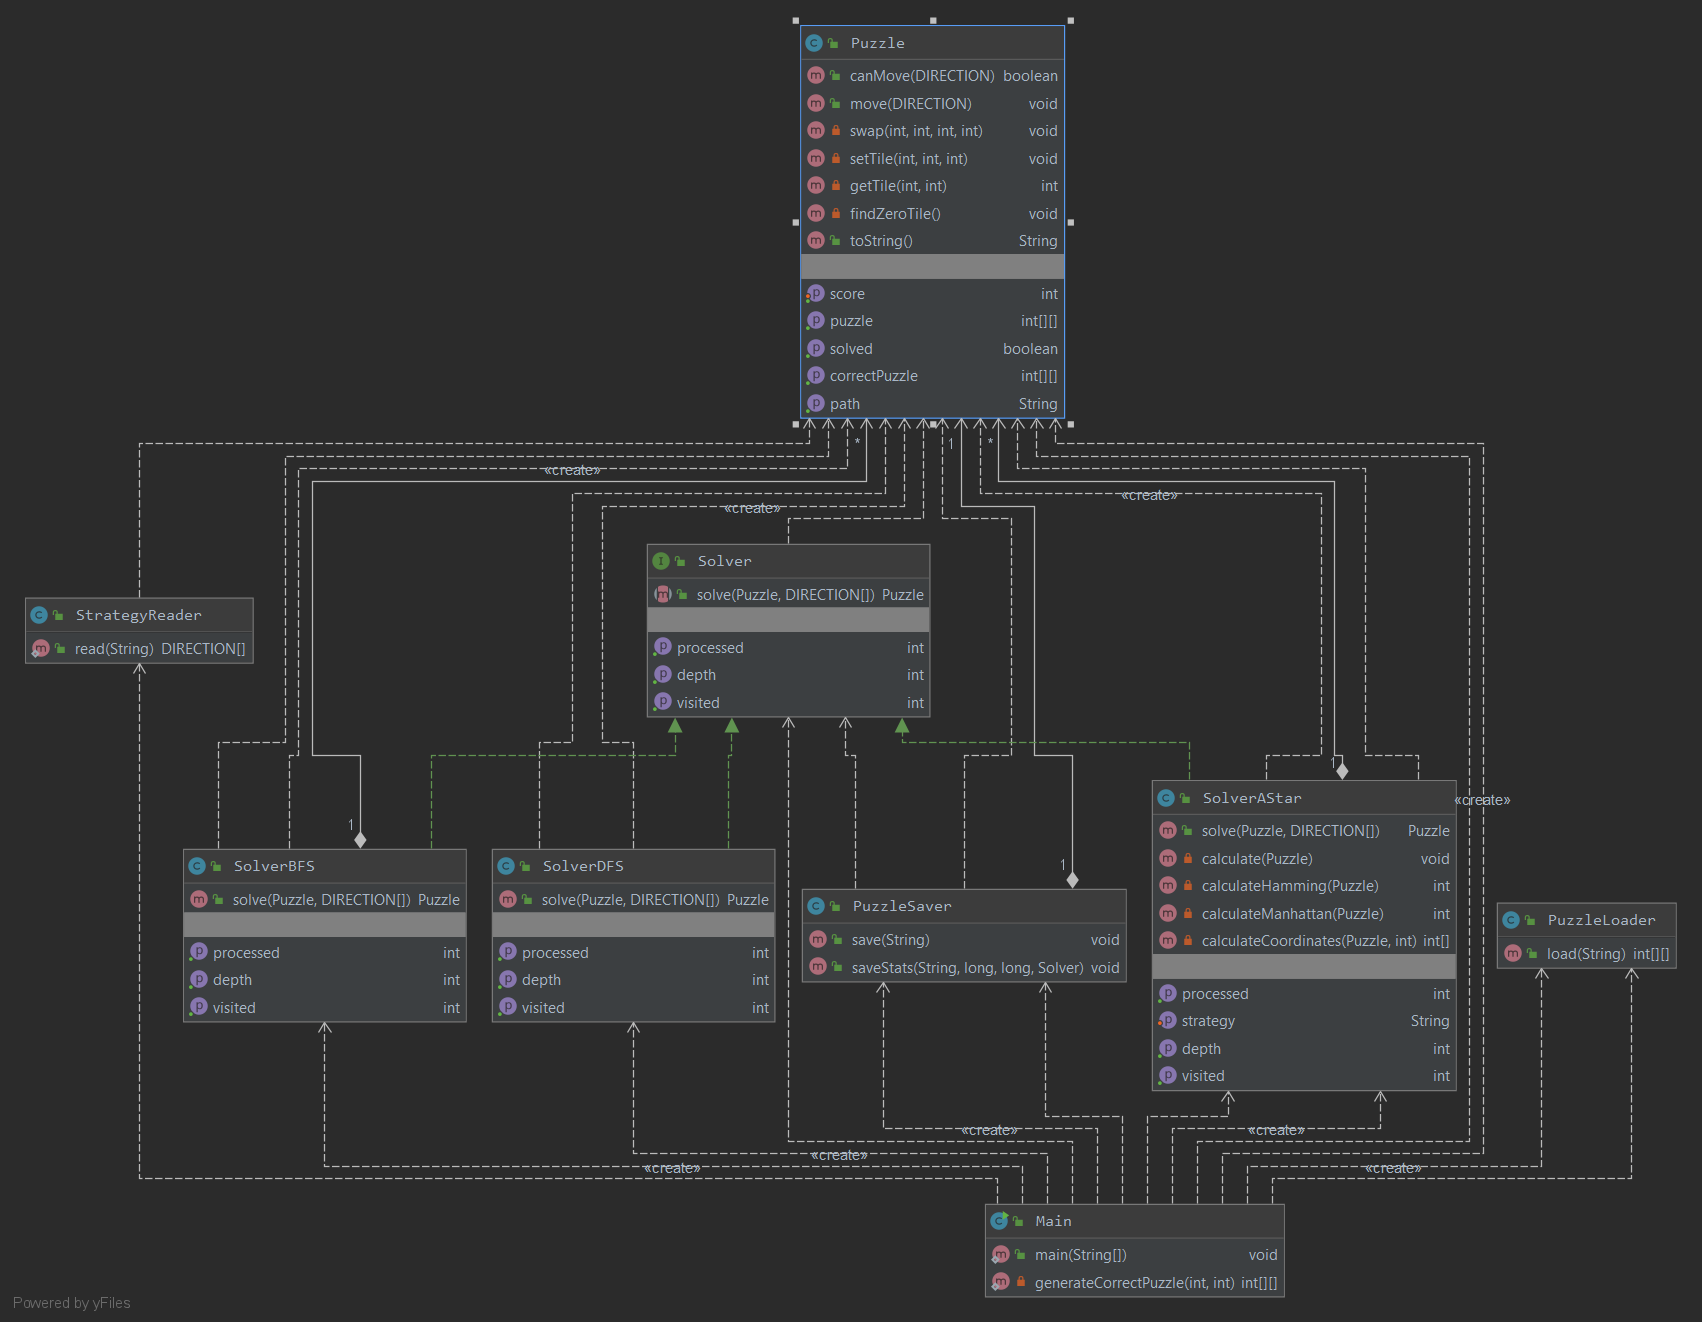
\includegraphics [scale=0.2]{SISE_Zad1_UML}
\caption{Diagram UML zawierający klasy aplikacji.}
\end{figure}


\section{Materiały i metody}
{Badania zostały przeprowadzone, na wszystkich możliwych układach do głębokości równej 7. W celu utworzenia tych układanek użyto generatora udostępnionego na platformie WIKAMP.
Następnie program uruchamiany jest dla każdej układanki i wszystkich możliwych strategii i parametrów je opisujących. Po otrzymaniu rezultatów dla wszystkich analizowanych przypadków, z utworzonych danych zostały stworzone wykresy, które zostaną przedstawionę w następnym punkcie sprawozdania. Ponieważ ilość analizowanych przypadków jest bardzo duża, w celu zebrania wszystkich danych i utworzenia odpowiednich wykresów napisano skrypt w języku python.}

\newpage
\section{Wyniki}
{
\begin{figure}[h]
\centering
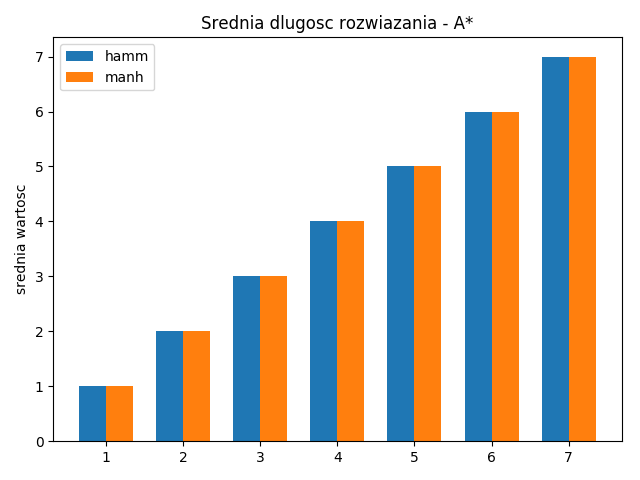
\includegraphics [scale=0.5]{dlugosc_AStar}
\caption{Wykres przedstawiający średnią długość rozwiązania dla strategii A*}
\end{figure}
\begin{figure}
\centering
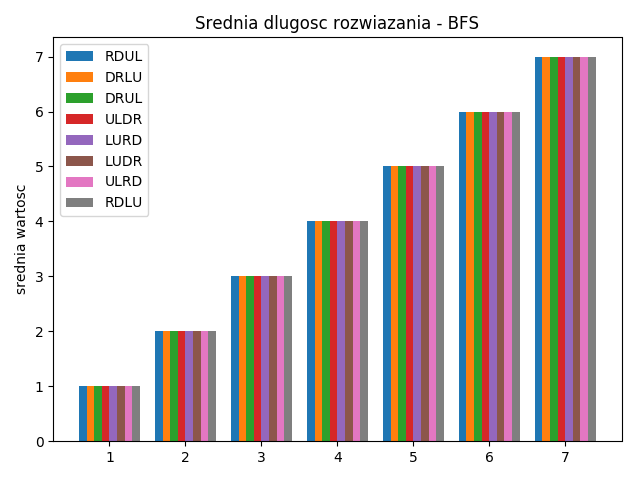
\includegraphics [scale=0.5]{dlugosc_BFS}
\caption{Wykres przedstawiający średnią długość rozwiązania dla strategii BFS}
\end{figure}
\begin{figure}
\centering
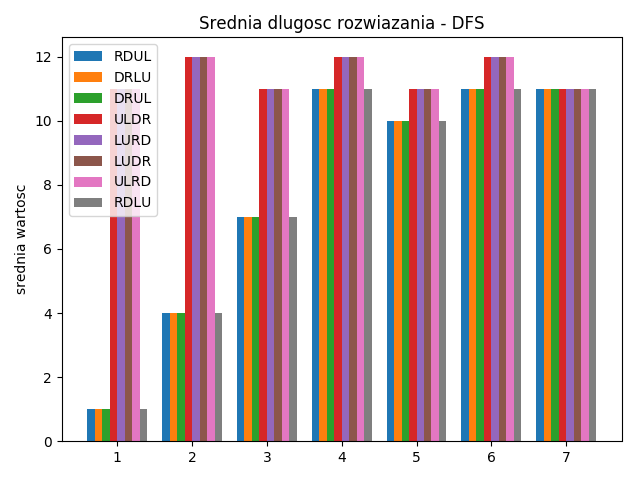
\includegraphics [scale=0.5]{dlugosc_DFS}
\caption{Wykres przedstawiający średnią ilość stanów odwiedzonych dla strategii DFS}
\end{figure}
\begin{figure}
\centering
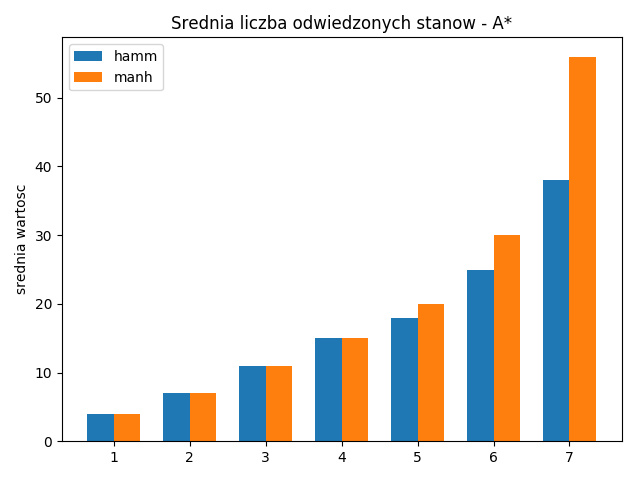
\includegraphics [scale=0.5]{odwiedzone_AStar}
\caption{Wykres przedstawiający średnią ilość stanów odwiedzonych dla strategii A*}
\end{figure}
\begin{figure}
\centering
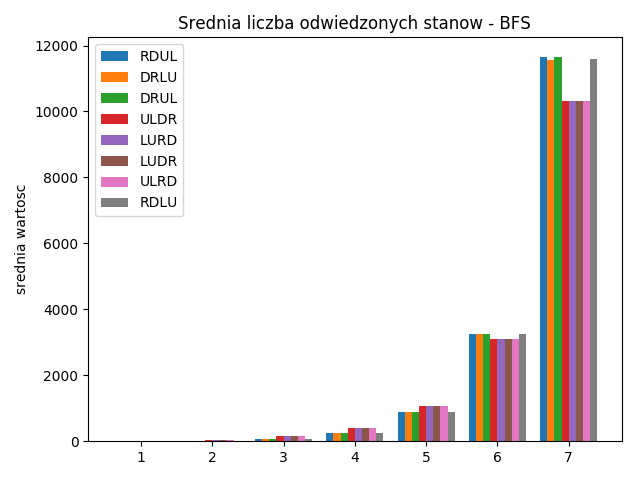
\includegraphics [scale=0.5]{odwiedzone_BFS}
\caption{Wykres przedstawiający średnią ilość stanów odwiedzonych dla strategii BFS}
\end{figure}
\begin{figure}
\centering
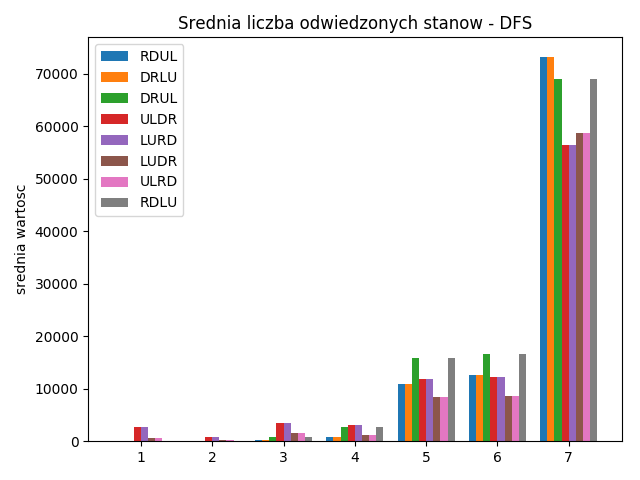
\includegraphics [scale=0.5]{odwiedzone_DFS}
\caption{Wykres przedstawiający średnią ilość stanów odwiedzonych dla strategii DFS}
\end{figure}
\begin{figure}
\centering
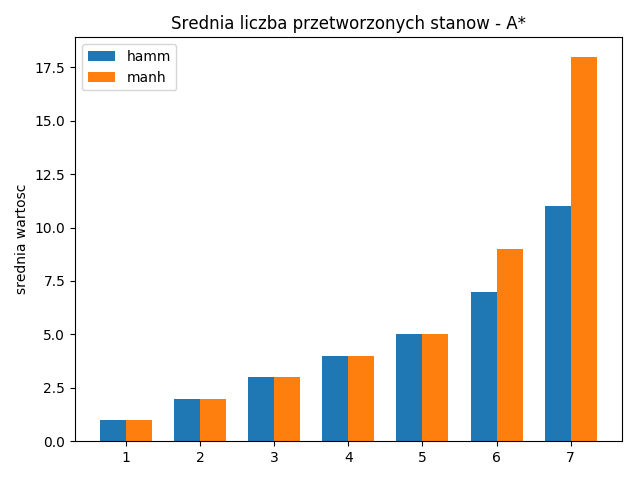
\includegraphics [scale=0.5]{przetworzone_AStar}
\caption{Wykres przedstawiający średnią ilość stanów przetworzonych dla strategii A*}
\end{figure}
\begin{figure}
\centering
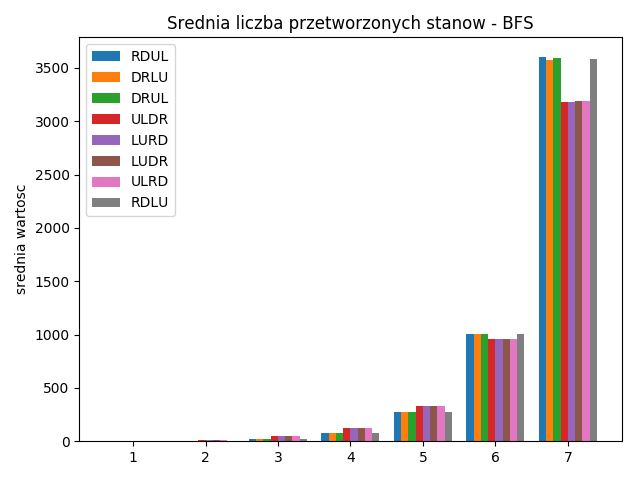
\includegraphics [scale=0.5]{przetworzone_BFS}
\caption{Wykres przedstawiający średnią ilość stanów przetworzonych dla strategii BFS}
\end{figure}
\begin{figure}
\centering
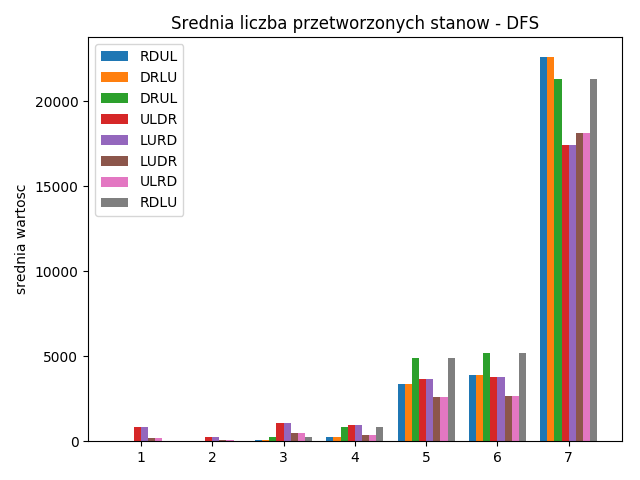
\includegraphics [scale=0.5]{przetworzone_DFS}
\caption{Wykres przedstawiający średnią ilość stanów przetworzonych dla strategii DFS}
\end{figure}
\begin{figure}
\centering
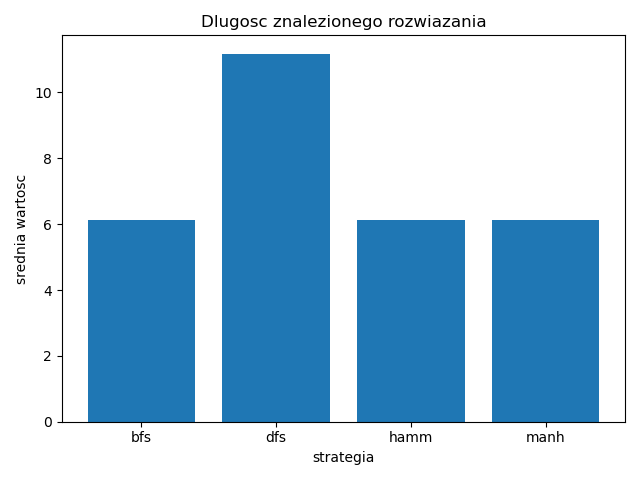
\includegraphics [scale=0.5]{dlugosc}
\caption{Wykres przedstawiający średnią długość rozwiązania dla wszystkich badanych strategii}
\end{figure}
\begin{figure}
\centering
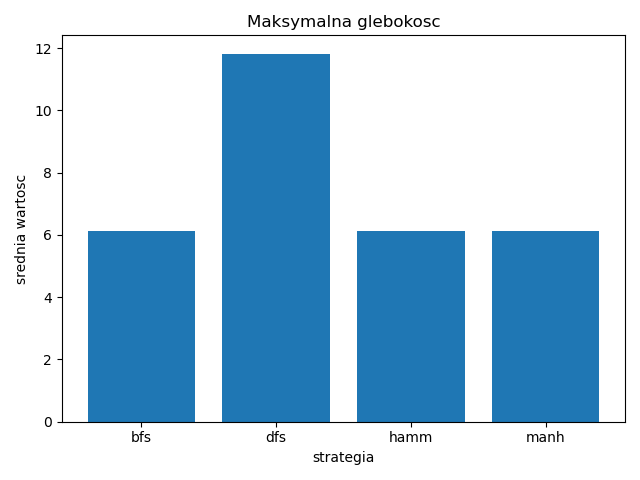
\includegraphics [scale=0.5]{glebokosc}
\caption{Wykres przedstawiający średnią maksymalną głębokość rozwiązania dla wszystkich badanych strategii}
\end{figure}
\begin{figure}
\centering
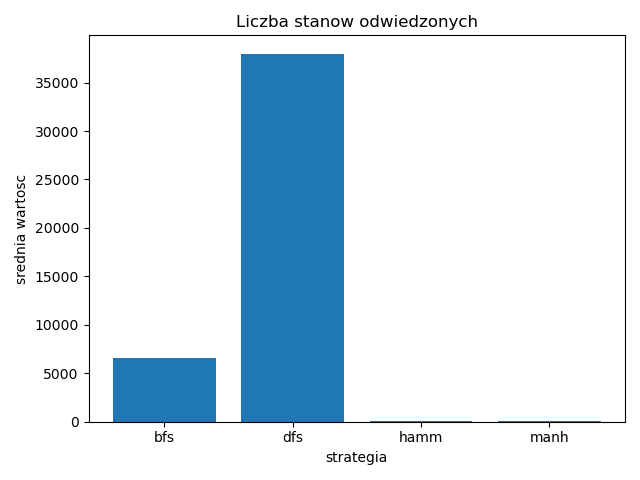
\includegraphics [scale=0.5]{odwiedzone}
\caption{Wykres przedstawiający średnią ilość stanów odwiedzonych dla wszystkich badanych strategii}
\end{figure}
\begin{figure}
\centering
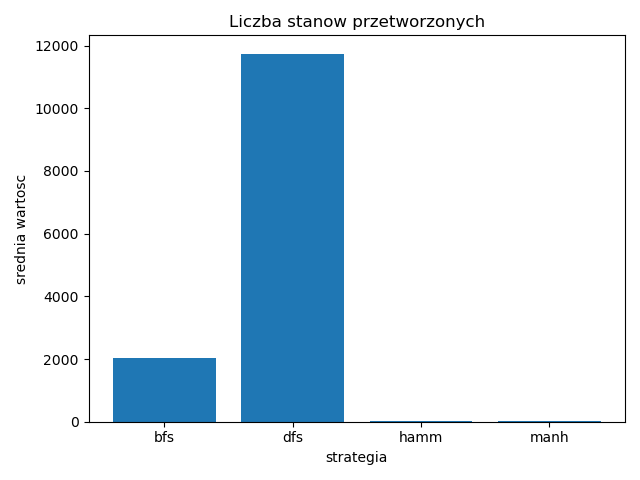
\includegraphics [scale=0.5]{przetworzone}
\caption{Wykres przedstawiający średnią ilość stanów przetworzonych dla wszystkich badanych strategii}
\end{figure}
}
\newpage
\section{Dyskusja}
{Omówmy wszystkie analizowane wartości.
\begin{enumerate}
\item{ Średnia długość rozwiązania:}
\newline Porównując cztery główne strategie widzimy, że w przypadku strategii DFS długość rozwiązania jest wyraźnie najdłuższa. Porównując dwie heurystki strategii A* widzimym, że średnie długości dla nich są niemal identyczne na wszystkich głebokościach. W przypadku strategii BFS wybór kolejności wykonywania ruchów (drugi argument programu) w żaden sposób nie wpływa na rozważaną wartość, w przeciwieństwie do strategii DFS gdzie widzimy że dla niektórych porządków wykonywania ruchów (np. ULDR i LURD) średnia długość rozwiązania już dla niskich głębokości przyjmuje wysokie wartości. W przypadku strategii BFS i A* można zauważyć, że wzrost długości rozwiązania do głębokości rozważanego układu rośnie mniej więcej liniowo, a w przypadku strategii DFS wzrost jest nieregularny.
\item {Średnia głębokość rozwiązania:}
\newline Wartości, które otrzymujemy na wykresie porównującym średnią maksymalną głębokość rozwiązania przyjmują niemalże identyczne proporcje jak wartości dotyczące długości znalezionego rozwiązania. Jedyną różnicą wartą odnotowania jest nieznaczne większe wartości przyjmowane w przypadku strategii DFS.
\item {Stany odwiedzone i przetworzone}
\newline Porównując rozważane strategie między sobą można wysunąć dwa następujące spostrzeżenia. Pierwsze to w jak bardzo znaczącym stopniu strategia DFS odbiega od pozostałych, tj. przyjmuje ona znacznie większe wartości niż pozostałe strategie. Drugie spostrzeżenie to że obie heurystyki rozważane dla strategii A* przyjmują radykalnie mniejsze wartości od strategii DFS i BFS. Analizując otrzymane wyniki dla strategii A* możemy zauważyć, że przy niskich wartościach głębokości układanek rezultaty otrzymane dla obu matryk (Hamminga i Manhattana) przyjmują bardzo zbliżone wartości. Jednak przy wyższych wartościach głębokości widzimy, że dla matryki Manhattana liczba przetworzonych i odwiedzonych stanów jest znacznie większa niż w przypadku metryki Hamminga, najbardziej jest to widoczne przy ostatniej rozważanej głębokości, czyli głębokości równej 7. W przypadku strategii BFS i DFS wzrost liczby odwiedzonych i przetworzonych stanów rośnie mniej więcej wykładniczo i jest porównywalny w obu strategiach. W przypadku strategii DFS widać większą różnicę pomiędzy różnymi porządkami wykonywania ruchów niż w przypadku strategii BFS.
\end{enumerate}
}

\newpage
\section{Wnioski}
\begin{enumerate}
\item Różnica liczb stanów odwiedzonych i przetworzonych dla poszczególnych algorytmów jest znacząca. Najgorzej w obu przypadkach wypada strategia przeszukiwania w głąb, gdzie względem najlepszego A* (w obu badanych metodykach) jest to różnica kilku rzędów wielkości.
\item W przypadku strategii A*obie rozważane metodyki prezentują podobną wydajność. Różnice można zauważyć w przypadku liczby odwiedzonych i przetworzonych stanów, szczególne przy większych głębokościach.
\item Zdecydowanie najgorzej wypadającą strategią znajdywania rozwiązania dla "Piętnastki" jest metoda przeszukiwania w głąb (DFS), która wypada najgorzej pod każdym badanym względem.
\item Za najwydajniesze rozwiązanie można uznać strategię A*. Obie zastosowane metodyki wykazały się znacznie lepszą wydajnością niż strategie \textit{brute force} - BFS i DFS.
\end{enumerate}

\begin{thebibliography}{0}
  \bibitem{l2short} T. Oetiker, H. Partl, I. Hyna, E. Schlegl.
    \textsl{Nie za krótkie wprowadzenie do systemu \LaTeX2e}, 2007, dostępny
    online.
  \bibitem{l2short} \url{https://en.wikipedia.org/wiki/A*_search_algorithm}
  \bibitem{l2short} \url{https://en.wikipedia.org/wiki/15_puzzle}
  
\end{thebibliography}
\end{document}
